\documentclass{beamer}

\usepackage{beamerthemeboxes}
\usepackage{listings}
\usepackage{color}

\definecolor{mygreen}{rgb}{0,0.6,0}
\definecolor{mygray}{rgb}{0.5,0.5,0.5}
\definecolor{mymauve}{rgb}{0.58,0,0.82}

\lstset{ %
  backgroundcolor=\color{white},   % choose the background color
  basicstyle=\footnotesize,        % size of fonts used for the code
  breaklines=true,                 % automatic line breaking only at whitespace
  captionpos=t,                    % sets the caption-position to bottom
  commentstyle=\color{mygreen},    % comment style
  escapeinside={\%*}{*)},          % if you want to add LaTeX within your code
  keywordstyle=\color{blue},       % keyword style
  stringstyle=\color{mymauve},     % string literal style
}



\title{Auto-vectorization}
\author[Adam Kosiorek]{Adam Kosiorek\\ \\{\tiny Supervised by: Prof. M. Gerndt}}
\date {June 3, 2015}

\begin{document}

\frame{\titlepage}

%\section*{Outline}
%\frame{\tableofcontents}

\section{Vectorization}

\begin{frame}[fragile]
  \frametitle{What is vectorization?}

  \begin{equation}
    Vectorization = {Loop\ unrolling} + {packed\ SIMD\ instructions}  
  \end{equation}
  
  Loop unrolling: manually or by compiler \\\ \\
  SIMD: SSE, AVX, Nano etc. \\\ \\
  How to get them:
  \begin{itemize}
   \item write assembly
   \item compiler intrinsics
   \item special purpose language extensions eg. OpenCL, CUDA
   \item vectorizing compiler + guidelines
  \end{itemize}
\end{frame}

\begin{frame}[fragile]
  \frametitle{The simplest case}
  
  \begin{lstlisting}[language=C++]
    double A[1024], B[1024], C[1024];
    // initialize A and B
    for(int i = 0; i < 1024; ++i) 
      C[i] = A[i] * B[i];   
  \end{lstlisting}
  
  \begin{columns}[onlytextwidth]
    \begin{column}{0.4\textwidth}
     \textbf{vectorized}:
     \begin{itemize}
      \item -O2 and beyond
      \item speedup $\in [2, 8]$
     \end{itemize}
    \end{column}
    
    \begin{column}{0.4\textwidth}
     \textbf{not vectorized}:
     \begin{itemize}
      \item -O0, -O1, -Og, -g, -no-vec
      \item operates on single entry at a time
      \item slow
     \end{itemize}
    \end{column}
  \end{columns}
  
\end{frame}


\begin{frame}[fragile]
  \frametitle{The simplest case - vectorization}
  
  \textbf{default}:
  \begin{lstlisting}[language=C++]
    for(i = 0; i < MAX; ++i) 
      C[i] = A[i] * B[i];   
  \end{lstlisting}
  
  \textbf{unrolled}:
  \begin{lstlisting}[language=C++]
    for(i = 0; i < MAX; i+=4) {
      C[i] = A[i] * B[i];
      C[i+1] = A[i+1] * B[i+2];
      C[i+2] = A[i+1] * B[i+2];
      C[i+3] = A[i+3] * B[i+3];
    }
  \end{lstlisting}
  
  \textbf{vectorized}: \textcolor{gray}{(with AVX intrinsics)}
  \begin{lstlisting}[language=C++]
    __m256* mA = (__m256*)A;
    __m256* mB = (__m256*)B;
    __m256* mC = (__m256*)C;
    for(i = 0; i < MAX/4; ++i) 
      mC[i] = _mm256_add_pd(mA[i], mB[i]);
  \end{lstlisting}
  
\end{frame}


\begin{frame}[fragile]
  \frametitle{Why was it vectorized?}
   \begin{columns}[onlytextwidth]
    \begin{column}{0.4\textwidth}
     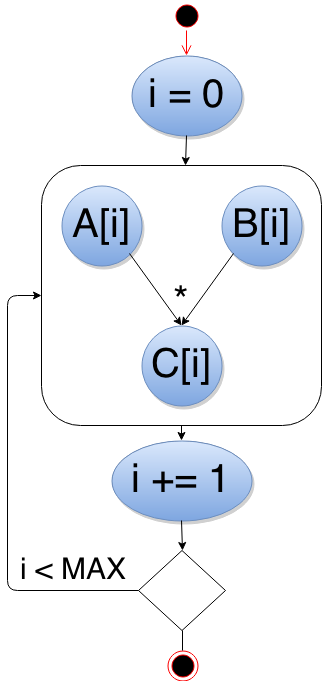
\includegraphics[width=0.75\textwidth]{countable}
    \end{column}
    
    \begin{column}{0.6\textwidth}
      Properties needed for vectorization:
      \begin{itemize}
      \item countable
      \item single entry, single exit
      \item no branching
      \item the innermost loop
      \item no function calls
      \item no data dependencies
      \end{itemize}
    \end{column}
  \end{columns}  
  
\end{frame}

\section{What can be vectorized?}

\begin{frame}[fragile]
  \frametitle{Countable}
    \begin{columns}[onlytextwidth]
      \begin{column}{0.5\textwidth}
	 \textbf{(a)} countable:
	 \begin{lstlisting}[language=C++]
	  for(i = 0; i < MAX; ++i) 
	    C[i] = A[i] * B[i];   
	\end{lstlisting}
      \end{column}
      \begin{column}{0.5\textwidth}
	\textbf{(b)} uncountable:
	\begin{lstlisting}[language=C++]
	  for(i = 0; i < MAX; ++i) 
	  {
	    C[i] = A[i] * B[i];
	    if(A[i] < B[i])
	      MAX--;
	   }
	\end{lstlisting}
      \end{column}
    \end{columns}
    
    Index cannot depend on the loop execution!   
\end{frame}

\begin{frame}[fragile]
  \frametitle{Single entry, single exit}
    \begin{columns}[onlytextwidth]
      \begin{column}{0.5\textwidth}
	 \textbf{(a)} single exit:
	 \begin{lstlisting}[language=C++]
	  for(i = 0; i < MAX; ++i) 
	    C[i] = A[i] * B[i];   
	\end{lstlisting}
      \end{column}
      \begin{column}{0.5\textwidth}
	\textbf{(b)} multiple exits:
	\begin{lstlisting}[language=C++]
	  for(i = 0; i < MAX; ++i) 
	  {
	    C[i] = A[i] * B[i];
	    if(A[i] < B[i])
	      break;
	   }
	\end{lstlisting}
      \end{column}
    \end{columns}
    
    Vectorization could ``skip'' the termination condition!
\end{frame}

\begin{frame}[fragile]
  \frametitle{No branching}
    \begin{columns}[onlytextwidth]
      \begin{column}{0.5\textwidth}
	 \textbf{(a)} no branching?:
	 \begin{lstlisting}[language=C++]
	  for(i = 0; i < MAX; ++i) 
	    if(A[i] != 0)
	      C[i] = A[i];
	    else
	      C[i] = B[i];
	\end{lstlisting}
      \end{column}
      \begin{column}{0.5\textwidth}
	\textbf{(b)} branching:
	\begin{lstlisting}[language=C++]
	  for(i = 0; i < MAX; ++i) 
	    switch(i % 3) {
	    case 0: C[i] = A[i]; 
	            break;
	    case 1: C[i] = B[i]; 
	            break;
	    default: C[i] = 0;
	    }
	\end{lstlisting}
      \end{column}
    \end{columns}
    
    If statements implemented by ``masking assignment'' are ok.
\end{frame}


\begin{frame}[fragile]
  \frametitle{Innermost loops}
    \begin{lstlisting}[language=C++]
	for(int i = 0; i < 10; ++i)
	  for(j = 0; j < MAX; ++j) 
	    C[i][j] = A[i][j] * B[i][j];   
    \end{lstlisting}
    \begin{itemize}
     \item Only j-loop vectorized
     \item Outer-loop vectorization inefficient
     \item Can be enforced with \#pragma SIMD
     \item Outer-loop vectorization possible after loop interchange
    \end{itemize}    
\end{frame}

\begin{frame}[fragile]
  \frametitle{Function Calls}
     
     \begin{lstlisting}[language=C++]
	int compute(int a, int b);
	...
	for(i = 0; i < MAX; ++i) 
	  C[i] = compute(A[i], B[i]);   
     \end{lstlisting}
    
    works if the function:
    \begin{itemize}
     \item can be inlined
     \item is declared as a vector function:
     \begin{lstlisting}[language=C++]
	__attribute__((vector))
	int compute(int a, int b);
     \end{lstlisting}

     \item is compiler intrinsic function
     \item is one of the math functions: sin, cos, exp, pow, etc.
    \end{itemize}    
\end{frame}

\section{Obstacles to vectorization}

\begin{frame}[fragile]
  \frametitle{Non-contiguous Memory Access}
  \begin{figure}
    \begin{center}
      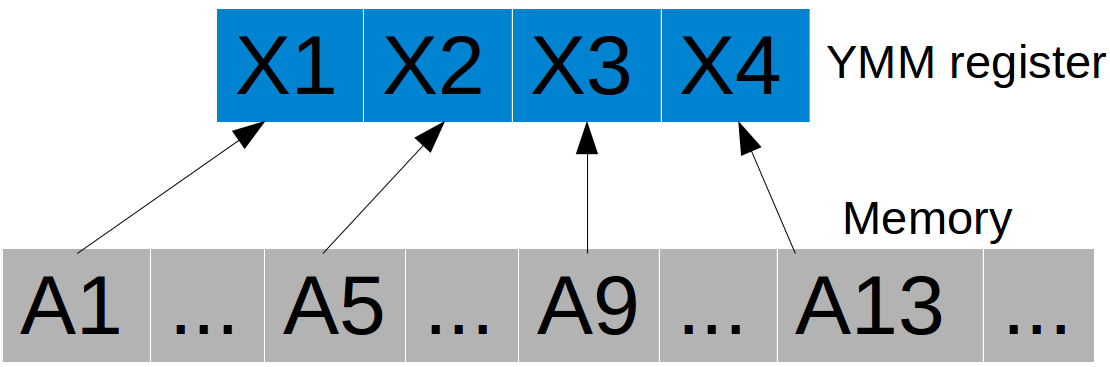
\includegraphics[width=0.75\textwidth]{non-contigous}
    \end{center}
  \end{figure}
  
  \begin{itemize}
   \item each entry loaded separately
   \item happens with non-unit stride and indirect adressing e.g.
   \begin{lstlisting}[language=C++]
    C[i] = C[i] * A[i * 2];
    C[i] = C[i] * A[B[i]];
   \end{lstlisting}

  \end{itemize}


  
\end{frame}

\begin{frame}[fragile]
  \frametitle{Data Dependencies}
  Read-after-write (flow dependency): \textcolor{red}{$\times$}
  \begin{lstlisting}[language=C++]
    for(i=1; i<MAX; ++i) 
      A[i] = A[i-1] + 1;
  \end{lstlisting}
  Write-after-read (anti-dependency): \textcolor{green}{\checkmark}
  \begin{lstlisting}[language=C++]
    for(i=1; i<MAX; ++i) 
      A[i-1] = A[i] + 1;
  \end{lstlisting}
  Write-after-write (output dependency): \textcolor{red}{$\times$}
  \begin{lstlisting}[language=C++]
   for(i=0; i<MAX; ++i)
     A[i - i%2] = A[i] * B[i]; 
  \end{lstlisting}
  Reduction: \textcolor{green}{\checkmark}
  \begin{lstlisting}[language=C++]
   double sum = 0;
   for(i=0; i<MAX; ++i)
     sum = sum + A[i];
  \end{lstlisting}
\end{frame}

\begin{frame}[fragile]
  \frametitle{Assumed Data Dependencies - Pointer Aliasing}
  \begin{lstlisting}[language=C++]
    void compute(int* A, int* B, int* C, int N) {
      for(int i = 0; i<N; ++i) 
        C[i] = A[i] + B[i];
    }
  \end{lstlisting}
  
  \begin{itemize}
   \item C/C++ makes no assumptions about pointers:
   \begin{lstlisting}[language=C++]
      compute(a, b, a);
  \end{lstlisting}
  is legal!
  \end{itemize}

  
  
  \begin{lstlisting}[language=C++]

  \end{lstlisting}
\end{frame}

\begin{frame} 
 \frametitle{References}
 \begin{enumerate}
  \item A Guide to Vectorization with Intel® C++ Compilers \url{https://software.intel.com/en-us/articles/a-guide-to-auto-vectorization-with-intel-c-compilers}
  \item Intel Intrinsics Guide \url{https://software.intel.com/sites/landingpage/IntrinsicsGuide/}
 \end{enumerate}

 

\end{frame}

\begin{frame} 
 Thank you for your attention
\end{frame}


\end{document}